\section{Self-improvement methods}
\label{app:methods}

\begin{table*}[h]
\centering
\small
\setlength{\tabcolsep}{4pt}
\begin{tabular}{@{}lp{5.3cm}p{3.9cm}p{2.8cm}@{}}
\toprule
Method & At test time & Learned on development tasks & In the spirit of \\
\midrule
\texttt{NoImprove} & one program, no feedback & -- & baseline \\
\texttt{SelfDebug} & retry with the error only; stop once the program runs & -- &
\citet{chen2024selfdebug} \\
\texttt{CheckFeedback} & retry with the failed checks, their causes and cards & -- &
verifier feedback \\
\texttt{Reflexion} & as \texttt{CheckFeedback}, plus a written reflection before each retry &
-- & \citet{shinn2023reflexion} \\
\texttt{PlaybookLearning} & as \texttt{CheckFeedback}, with a frozen playbook in the prompt &
playbook entries, through the gated loop & \citet{zhao2024expel,suzgun2026dynamic} \\
\texttt{Team} & a writer and one reviewer per rule family, from the same model & -- &
multi-role review \\
\texttt{Evolve} & as \texttt{CheckFeedback}, with an evolved prompt addendum & the addendum,
over \EvolveGenerations{} generations on \EvolveMinibatch{} tasks & \citet{agrawal2026gepa} \\
\bottomrule
\end{tabular}
\caption{The \NMethods{} self-improvement methods. All share the prompt, the judge and the
budget; each keeps the mechanism it is known for. They are not reproductions of the original
systems.}
\label{tab:methods}
\end{table*}

\texttt{Reflexion} asks for a reflection of at most five sentences, without code, and keeps
the reflections for the rest of the episode. In \texttt{Team}, a reviewer is asked only when a
check of its own family failed; it sees the program, the failed checks, their causes and its
family's cards, and answers with a diagnosis rather than code. \texttt{Evolve} rewrites a
prompt addendum of at most 1,200 characters from the visible failures of the current best
addendum, and keeps a candidate only if it scores strictly higher on the same development
tasks. The playbook is a list of short entries on three surfaces (tool usage, retrieval,
experience). Its loop rejects whitespace-only and repeated edits, and appends every proposal,
evaluation and decision to a journal whose receipts carry evidence hashes; a frozen playbook
cannot change. A stricter \emph{all-pass} rule, which vetoes any candidate while a single
task fails, blocks learning for a weak model, so we use no-regression.

\begin{figure*}[t]
\centering
\resizebox{\textwidth}{!}{% Figure: the gated playbook loop of PlaybookLearning, told in pictures. The halves are the
% development and validation splits of the development tasks (split by algorithm), and the gate is
% guard_rule="no_regression" in fin_skills/rsi/core.py: accept only if neither half scores lower,
% one scores higher and no task that passed its checks now fails. The dots are an example, not
% results. The proposal budget is a macro from numbers.tex.
\InputIfFileExists{figures/glyphs}{}{% Glyphs for the method figures (episode, gate, arms). Pictures first, words only as labels.%
% Colours, text styles, lines, corners, shadows and arrows come from figures/figstyle.tex,%
% icons from figures/lucide.tex. Load figstyle if the document has not.%
\ifcsname figTitleFont\endcsname\else\InputIfFileExists{figures/figstyle}{}{% The one figure style of the Fin-RSI paper, shared by every TikZ figure and every version
% (ACL draft, FinFM 7 and 4 pages). make_figures.py and make_results.py read the colours below
% through figstyle.py, so the data figures cannot drift from the diagrams.
%
% Rules: figures are drawn at print size and never scaled; no text below 7 pt; one meaning per
% colour (skills and the library blue, checks orange, self-improvement aqua, pass and fail green
% and red with a mark); icons are Lucide (figures/lucide.tex), one icon per meaning.
%
% Palette: the reference palette's first slots, validated for colour vision deficiency.
\definecolor{finblue}{HTML}{2A78D6}%     skills, rule cards, the library
\definecolor{finorange}{HTML}{EB6834}%   checks
\definecolor{finaqua}{HTML}{1BAF7A}%     self-improvement
\definecolor{finmagenta}{HTML}{C2408B}%  fourth slot, spare
% Neutrals: one cool grey scale for text, lines and fills.
\definecolor{figink}{HTML}{1F2335}%      titles and labels
\definecolor{fingray}{HTML}{5A6374}%     secondary marks (the engine)
\definecolor{figmid}{HTML}{6A7385}%      notes, flow arrows, axes
\definecolor{figline}{HTML}{C9D0DA}%     outlines, unpicked items
\definecolor{figfaint}{HTML}{EEF1F5}%    empty cells, light fills
% Status: only with a check or a cross.
\definecolor{figok}{HTML}{1E9E6A}%
\definecolor{figbad}{HTML}{D2483E}%
% Older names, kept so every figure file reads the same colours.
\colorlet{gink}{figink}\colorlet{gmid}{figmid}\colorlet{gline}{figline}%
\colorlet{gok}{figok}\colorlet{gbad}{figbad}%
\colorlet{kink}{figink}\colorlet{kuse}{figmid}\colorlet{koff}{figline}%
%
% Text: four levels, plus the typewriter face of the body for code.
\providecommand{\figTitleFont}{\sffamily\bfseries\fontsize{7.5}{9}\selectfont}%
\providecommand{\figLabelFont}{\sffamily\fontsize{7.5}{9}\selectfont}%
\providecommand{\figSmallFont}{\sffamily\fontsize{7}{8.4}\selectfont}%
\providecommand{\figBrandFont}{\sffamily\bfseries\fontsize{8.4}{10}\selectfont}%
\providecommand{\figCodeFont}{\ttfamily\fontsize{7}{8.6}\selectfont}%
\providecommand{\glab}{\fontsize{7.5}{9}\selectfont}%
\providecommand{\gsmall}{\fontsize{7}{8.4}\selectfont}%
%
\InputIfFileExists{figures/lucide}{}{\input{../latex_acl2027/figures/lucide}}%
\tikzset{%
  fig title/.style={font=\figTitleFont, text=figink, inner sep=0},%
  fig label/.style={font=\figLabelFont, text=figink, inner sep=0, align=center},%
  fig small/.style={font=\figSmallFont, text=figink!85, inner sep=0, align=center},%
  fig note/.style={font=\figSmallFont, text=figmid, inner sep=0, align=center},%
  fig code/.style={font=\figCodeFont, text=figink, inner sep=0},%
  % lines: 0.5 pt outlines, 0.7 pt icons (lucide), 0.8 pt arrows
  fig outline/.style={line width=0.5pt},%
  fig shadow/.style={blur shadow={shadow blur steps=6, shadow xshift=0pt,%
    shadow yshift=-0.8pt, shadow opacity=16, shadow blur radius=1.8pt}},%
  % corners: 1 pt items, 2.5 pt cards and compartments, 4 pt containers
  fig item/.style={rounded corners=1pt},%
  fig card/.style={fill=white, draw=figline, line width=0.5pt, rounded corners=2.5pt, fig shadow},%
  fig box/.style={fill=white, draw=figline, line width=0.5pt, rounded corners=4pt, fig shadow},%
  % arrows: one tip, four meanings
  fig arrow/.style={-{Latex[length=1.6mm,width=1.4mm]}, line width=0.8pt},%
  fig flow/.style={fig arrow, draw=figmid!70},%
  fig pass/.style={fig arrow, draw=figok},%
  fig fail/.style={fig arrow, draw=figbad!80, dash pattern=on 3pt off 1.8pt},%
  fig back/.style={fig arrow, draw=finaqua!85!black},%
  % names the figure files already use
  gword/.style={fig label},%
  gnote/.style={fig note},%
  gflow/.style={fig flow},%
  gshade/.style={fig shadow},%
}%
}\fi%
% \gpage{centre}{w}{h}{fill}: a page with a folded corner.%
\providecommand{\gpage}[4]{%
  \begin{scope}[shift={#1}]%
    \path[fill=#4, draw=gline, line width=0.5pt, line join=round, gshade]%
      ({-#2/2},{-#3/2}) -- ({#2/2},{-#3/2}) -- ({#2/2},{#3/2-0.2}) -- ({#2/2-0.2},{#3/2}) -- ({-#2/2},{#3/2}) -- cycle;%
    \draw[gline, line width=0.5pt, line join=round, fill=gline!40] ({#2/2-0.2},{#3/2}) -- ({#2/2-0.2},{#3/2-0.2}) -- ({#2/2},{#3/2-0.2});%
  \end{scope}}%
% \gbar{x0}{y}{length}{colour}: one line of text or code, drawn as a rounded bar.%
\providecommand{\gbar}[4]{\draw[#4, line width=2.4pt, line cap=round] (#1,#2) -- ({#1+#3},#2);}%
% \gcheck{centre}{state}: a check that passed (1) or failed (0), Lucide check or x on a disc.%
\providecommand{\gcheck}[2]{%
  \ifnum#2=1 \fill[figok] #1 circle (0.13);%
    \pic[draw=white, line width=0.85pt, scale=0.62] at #1 {lu check};%
  \else \fill[figbad] #1 circle (0.13);%
    \pic[draw=white, line width=0.85pt, scale=0.62] at #1 {lu x};\fi}%
% \gcard{centre}: a rule card, small and blue.%
\providecommand{\gcard}[1]{%
  \begin{scope}[shift={#1}]%
    \path[fill=finblue!12, draw=finblue!70, line width=0.55pt, fig item, gshade] (-0.22,-0.16) rectangle (0.22,0.16);%
    \draw[finblue!70, line width=0.9pt, line cap=round] (-0.13,0.05) -- (0.13,0.05) (-0.13,-0.05) -- (0.06,-0.05);%
  \end{scope}}%
% \glock{centre}: a padlock (Lucide lock) on a white disc, so it can sit on a line.%
\providecommand{\glock}[1]{%
  \fill[white] #1 circle (0.19);%
  \pic[draw=figink!80, line width=0.95pt, scale=1.05] at #1 {lu lock};}%
% \gbot{centre}{radius}: the model, a dark disc with the Lucide bot icon.%
\providecommand{\gbot}[2]{%
  \path[fill=figink, fig shadow] #1 circle (#2);%
  \pic[draw=white, line width=0.75pt, scale={4.2*#2}] at #1 {lu bot};}%
}%
\begin{tikzpicture}[x=1cm, y=1cm, font=\sffamily]
\def\Y{1.35}
\def\book#1#2{% \book{centre x}{colour of the new entry, or n for none}
  \gpage{(#1+0.1,\Y+0.08)}{1.0}{1.2}{white}
  \gpage{(#1,\Y)}{1.0}{1.2}{white}
  \foreach \k/\l in {1/0.62, 2/0.5, 3/0.66} {\gbar{#1-0.36}{\Y+0.36-0.18*\k}{\l}{gline}}
  \ifx#2n\else\gbar{#1-0.36}{\Y+0.36-0.18*4}{0.56}{#2}\fi}
\def\tasks#1#2#3{% \tasks{x}{y}{how many of 4 passed}
  \foreach \i in {1,...,4} {
    \ifnum\i>#3 \draw[gmid!70, line width=0.5pt] ({#1+0.2*(\i-1)},#2) circle (0.062);
    \else \fill[gok] ({#1+0.2*(\i-1)},#2) circle (0.068);\fi}}
% ---------------------------------------------------------------- playbook, proposer, candidate
\book{1.05}{n}
\node[gword] at (1.05,\Y-0.88) {playbook P};
\node[gnote] at (1.05,\Y-1.15) {in every prompt};
\draw[gflow] (1.72,\Y) -- (3.15,\Y);
\gbot{(3.65,\Y)}{0.33}
\node[gword] at (3.65,\Y-0.88) {proposer};
\node[gnote] at (3.65,\Y-1.15) {sees checks, not grades};
\draw[gflow] (4.1,\Y) -- (5.55,\Y);
\book{6.25}{gok}
\node[gword] at (6.25,\Y-0.88) {candidate P$'$};
\node[gnote] at (6.25,\Y-1.15) {one entry added};
\draw[gflow] (6.92,\Y) -- (7.5,\Y);
% ---------------------------------------------------------------- two halves
\begin{scope}[shift={(7.62,0)}]
  \path[fill=white, draw=gline, line width=0.5pt, rounded corners=2pt, gshade] (0,\Y-0.62) rectangle (3.3,\Y+0.62);
  \draw[gline, line width=0.5pt] (1.73,\Y-0.5) -- (1.73,\Y+0.5);
  \node[gnote, anchor=east] at (0.34,\Y+0.2) {P};
  \node[gnote, anchor=east] at (0.34,\Y-0.2) {P$'$};
  \tasks{0.5}{\Y+0.2}{3} \tasks{0.5}{\Y-0.2}{3}
  \tasks{2.05}{\Y+0.2}{2} \tasks{2.05}{\Y-0.2}{3}
  \node[gword] at (0.86,\Y-0.88) {development};
  \node[gword] at (2.42,\Y-0.88) {validation};
  \node[gnote] at (0.86,\Y-1.15) {same};
  \node[gnote] at (2.42,\Y-1.15) {higher};
\end{scope}
\draw[gflow] (10.98,\Y) -- (11.88,\Y);
% ---------------------------------------------------------------- the gate
\path[fill=white, draw=gink, line width=0.7pt, gshade] (12.45,\Y+0.5) -- (12.97,\Y) -- (12.45,\Y-0.5) -- (11.93,\Y) -- cycle;
\gcheck{(12.45,\Y)}{1}
\node[gword] at (12.45,\Y-0.88) {no-regression gate};
\node[gnote] at (12.45,\Y-1.15) {no half lower, one higher};
% accept: P' becomes the playbook
\draw[-{Latex[length=1.7mm,width=1.4mm]}, gok, line width=0.9pt] (12.45,\Y+0.52) .. controls (12.45,\Y+1.6) and (1.05,\Y+1.6) .. (1.05,\Y+0.74);
\node[gnote, fill=white, inner sep=1pt, text=gok!80!black] at (6.75,\Y+1.33) {accept: P$'$ becomes P};
% reject: P stays
\draw[-{Latex[length=1.7mm,width=1.4mm]}, gbad!80, line width=0.9pt] (12.99,\Y) -- (14.42,\Y);
\begin{scope}[opacity=0.55]\book{15.1}{gok}\end{scope}
\draw[gbad, line width=1.2pt, line cap=round] (14.75,\Y-0.4) -- (15.45,\Y+0.4) (14.75,\Y+0.4) -- (15.45,\Y-0.4);
\node[gword] at (15.1,\Y-0.88) {reject};
\node[gnote] at (15.1,\Y-1.15) {P stays};
\node[gnote, anchor=east] at (15.95,\Y+1.05) {at most \FitProposals{} proposals};
\end{tikzpicture}
}
\caption{The gated playbook loop of \texttt{PlaybookLearning}. The proposer reads development
traces without grades and adds one entry; the current and the candidate playbook are scored on
two disjoint halves of the development tasks (dots: tasks that passed their checks; an example,
not results). The no-regression gate accepts the candidate only if neither half is lower, one is
higher and no task that passed before now fails.}
\label{fig:gate}
\end{figure*}

\section{Experiment design}
\label{app:design}

\begin{figure}[h]
\centering
% Figure: the skill arms (rsi.ARMS) and the method contrasts of the component ablation, in
% pictures. A blue card stands for the rule cards and a dark square for the library interface;
% faint means the arm leaves it out. Bold frames are the arms of the main comparison.
\InputIfFileExists{figures/glyphs}{}{% Glyphs for the method figures (episode, gate, arms). Pictures first, words only as labels.%
% Colours, text styles, lines, corners, shadows and arrows come from figures/figstyle.tex,%
% icons from figures/lucide.tex. Load figstyle if the document has not.%
\ifcsname figTitleFont\endcsname\else\InputIfFileExists{figures/figstyle}{}{% The one figure style of the Fin-RSI paper, shared by every TikZ figure and every version
% (ACL draft, FinFM 7 and 4 pages). make_figures.py and make_results.py read the colours below
% through figstyle.py, so the data figures cannot drift from the diagrams.
%
% Rules: figures are drawn at print size and never scaled; no text below 7 pt; one meaning per
% colour (skills and the library blue, checks orange, self-improvement aqua, pass and fail green
% and red with a mark); icons are Lucide (figures/lucide.tex), one icon per meaning.
%
% Palette: the reference palette's first slots, validated for colour vision deficiency.
\definecolor{finblue}{HTML}{2A78D6}%     skills, rule cards, the library
\definecolor{finorange}{HTML}{EB6834}%   checks
\definecolor{finaqua}{HTML}{1BAF7A}%     self-improvement
\definecolor{finmagenta}{HTML}{C2408B}%  fourth slot, spare
% Neutrals: one cool grey scale for text, lines and fills.
\definecolor{figink}{HTML}{1F2335}%      titles and labels
\definecolor{fingray}{HTML}{5A6374}%     secondary marks (the engine)
\definecolor{figmid}{HTML}{6A7385}%      notes, flow arrows, axes
\definecolor{figline}{HTML}{C9D0DA}%     outlines, unpicked items
\definecolor{figfaint}{HTML}{EEF1F5}%    empty cells, light fills
% Status: only with a check or a cross.
\definecolor{figok}{HTML}{1E9E6A}%
\definecolor{figbad}{HTML}{D2483E}%
% Older names, kept so every figure file reads the same colours.
\colorlet{gink}{figink}\colorlet{gmid}{figmid}\colorlet{gline}{figline}%
\colorlet{gok}{figok}\colorlet{gbad}{figbad}%
\colorlet{kink}{figink}\colorlet{kuse}{figmid}\colorlet{koff}{figline}%
%
% Text: four levels, plus the typewriter face of the body for code.
\providecommand{\figTitleFont}{\sffamily\bfseries\fontsize{7.5}{9}\selectfont}%
\providecommand{\figLabelFont}{\sffamily\fontsize{7.5}{9}\selectfont}%
\providecommand{\figSmallFont}{\sffamily\fontsize{7}{8.4}\selectfont}%
\providecommand{\figBrandFont}{\sffamily\bfseries\fontsize{8.4}{10}\selectfont}%
\providecommand{\figCodeFont}{\ttfamily\fontsize{7}{8.6}\selectfont}%
\providecommand{\glab}{\fontsize{7.5}{9}\selectfont}%
\providecommand{\gsmall}{\fontsize{7}{8.4}\selectfont}%
%
\InputIfFileExists{figures/lucide}{}{\input{../latex_acl2027/figures/lucide}}%
\tikzset{%
  fig title/.style={font=\figTitleFont, text=figink, inner sep=0},%
  fig label/.style={font=\figLabelFont, text=figink, inner sep=0, align=center},%
  fig small/.style={font=\figSmallFont, text=figink!85, inner sep=0, align=center},%
  fig note/.style={font=\figSmallFont, text=figmid, inner sep=0, align=center},%
  fig code/.style={font=\figCodeFont, text=figink, inner sep=0},%
  % lines: 0.5 pt outlines, 0.7 pt icons (lucide), 0.8 pt arrows
  fig outline/.style={line width=0.5pt},%
  fig shadow/.style={blur shadow={shadow blur steps=6, shadow xshift=0pt,%
    shadow yshift=-0.8pt, shadow opacity=16, shadow blur radius=1.8pt}},%
  % corners: 1 pt items, 2.5 pt cards and compartments, 4 pt containers
  fig item/.style={rounded corners=1pt},%
  fig card/.style={fill=white, draw=figline, line width=0.5pt, rounded corners=2.5pt, fig shadow},%
  fig box/.style={fill=white, draw=figline, line width=0.5pt, rounded corners=4pt, fig shadow},%
  % arrows: one tip, four meanings
  fig arrow/.style={-{Latex[length=1.6mm,width=1.4mm]}, line width=0.8pt},%
  fig flow/.style={fig arrow, draw=figmid!70},%
  fig pass/.style={fig arrow, draw=figok},%
  fig fail/.style={fig arrow, draw=figbad!80, dash pattern=on 3pt off 1.8pt},%
  fig back/.style={fig arrow, draw=finaqua!85!black},%
  % names the figure files already use
  gword/.style={fig label},%
  gnote/.style={fig note},%
  gflow/.style={fig flow},%
  gshade/.style={fig shadow},%
}%
}\fi%
% \gpage{centre}{w}{h}{fill}: a page with a folded corner.%
\providecommand{\gpage}[4]{%
  \begin{scope}[shift={#1}]%
    \path[fill=#4, draw=gline, line width=0.5pt, line join=round, gshade]%
      ({-#2/2},{-#3/2}) -- ({#2/2},{-#3/2}) -- ({#2/2},{#3/2-0.2}) -- ({#2/2-0.2},{#3/2}) -- ({-#2/2},{#3/2}) -- cycle;%
    \draw[gline, line width=0.5pt, line join=round, fill=gline!40] ({#2/2-0.2},{#3/2}) -- ({#2/2-0.2},{#3/2-0.2}) -- ({#2/2},{#3/2-0.2});%
  \end{scope}}%
% \gbar{x0}{y}{length}{colour}: one line of text or code, drawn as a rounded bar.%
\providecommand{\gbar}[4]{\draw[#4, line width=2.4pt, line cap=round] (#1,#2) -- ({#1+#3},#2);}%
% \gcheck{centre}{state}: a check that passed (1) or failed (0), Lucide check or x on a disc.%
\providecommand{\gcheck}[2]{%
  \ifnum#2=1 \fill[figok] #1 circle (0.13);%
    \pic[draw=white, line width=0.85pt, scale=0.62] at #1 {lu check};%
  \else \fill[figbad] #1 circle (0.13);%
    \pic[draw=white, line width=0.85pt, scale=0.62] at #1 {lu x};\fi}%
% \gcard{centre}: a rule card, small and blue.%
\providecommand{\gcard}[1]{%
  \begin{scope}[shift={#1}]%
    \path[fill=finblue!12, draw=finblue!70, line width=0.55pt, fig item, gshade] (-0.22,-0.16) rectangle (0.22,0.16);%
    \draw[finblue!70, line width=0.9pt, line cap=round] (-0.13,0.05) -- (0.13,0.05) (-0.13,-0.05) -- (0.06,-0.05);%
  \end{scope}}%
% \glock{centre}: a padlock (Lucide lock) on a white disc, so it can sit on a line.%
\providecommand{\glock}[1]{%
  \fill[white] #1 circle (0.19);%
  \pic[draw=figink!80, line width=0.95pt, scale=1.05] at #1 {lu lock};}%
% \gbot{centre}{radius}: the model, a dark disc with the Lucide bot icon.%
\providecommand{\gbot}[2]{%
  \path[fill=figink, fig shadow] #1 circle (#2);%
  \pic[draw=white, line width=0.75pt, scale={4.2*#2}] at #1 {lu bot};}%
}%
\begin{tikzpicture}[x=1cm, y=1cm, font=\sffamily]
\def\lib#1#2{% \lib{centre}{on 1 / off 0}: the library, a code square
  \begin{scope}[shift={#1}]
    \ifnum#2=1 \path[fill=gink, rounded corners=1.5pt, gshade] (-0.2,-0.2) rectangle (0.2,0.2);
      \pic[draw=white, line width=0.6pt, scale=0.72] at (0,0) {lu code};
    \else \draw[gline, line width=0.6pt, dash pattern=on 1.5pt off 1pt, rounded corners=1.5pt] (-0.2,-0.2) rectangle (0.2,0.2);\fi
  \end{scope}}
\def\crd#1#2{% \crd{centre}{on 1 / off 0}: the rule cards
  \ifnum#2=1 \gcard{#1}\else
  \begin{scope}[shift={#1}]\draw[gline, line width=0.6pt, dash pattern=on 1.5pt off 1pt, rounded corners=1pt] (-0.22,-0.16) rectangle (0.22,0.16);\end{scope}\fi}
\def\arm#1#2#3#4#5{% \arm{x}{y}{cards}{library}{main 1/0}
  \ifnum#5=1 \path[fill=white, draw=gink, line width=0.9pt, rounded corners=2pt, gshade] ({#1-0.75},{#2-0.36}) rectangle ({#1+0.75},{#2+0.36});
  \else \path[fill=white, draw=gline, line width=0.5pt, rounded corners=2pt, gshade] ({#1-0.75},{#2-0.36}) rectangle ({#1+0.75},{#2+0.36});\fi
  \crd{({#1-0.3},#2)}{#3} \lib{({#1+0.32},#2)}{#4}}
\tikzset{both/.style={gflow, {Latex[length=1.6mm,width=1.4mm]}-{Latex[length=1.6mm,width=1.4mm]}}}
% ---------------------------------------------------------------- (a) skill arms
\node[gword, anchor=west, font=\sffamily\glab\bfseries] at (0,3.85) {(a) Skill arms};
\node[gnote] at (2.6,3.48) {no library}; \node[gnote] at (5.0,3.48) {library};
\node[gnote, anchor=east] at (1.7,2.95) {no cards}; \node[gnote, anchor=east] at (1.7,1.75) {rule cards};
\arm{2.6}{2.95}{0}{0}{0} \arm{5.0}{2.95}{0}{1}{0}
\arm{2.6}{1.75}{1}{0}{1} \arm{5.0}{1.75}{1}{1}{1}
\draw[both] (3.4,2.95) -- (4.2,2.95);
\draw[both] (3.4,1.75) -- (4.2,1.75);
\draw[both] (2.6,2.55) -- (2.6,2.15);
\draw[both] (5.0,2.55) -- (5.0,2.15);
\draw[gink, line width=0.9pt, rounded corners=1pt] (4.42,3.78) rectangle ++(0.16,0.14);
\node[gnote, anchor=west] at (4.66,3.85) {main comparison};
% ---------------------------------------------------------------- (b) method contrasts
\node[gword, anchor=west, font=\sffamily\glab\bfseries] at (0,0.95) {(b) Within one arm};
\begin{scope}[shift={(0.9,0.05)}]
  \gpage{(0,0)}{0.5}{0.62}{white}
\end{scope}
\node[gword, font=\figCodeFont] at (0.9,-0.55) {NoImprove};
\node[gnote] at (0.9,-0.8) {one program};
\begin{scope}[shift={(3.65,0.05)}]
  \gpage{(0,0)}{0.5}{0.62}{white}
  \draw[-{Latex[length=1.4mm,width=1.2mm]}, gbad!75, line width=0.8pt, dash pattern=on 2pt off 1.3pt] (0.3,0.12) .. controls (0.75,0.55) and (-0.75,0.55) .. (-0.3,0.12);
  \gcheck{(0.46,-0.18)}{0}
\end{scope}
\node[gword, font=\figCodeFont] at (3.65,-0.55) {CheckFeedback};
\node[gnote] at (3.65,-0.8) {retries on failed checks};
\begin{scope}[shift={(6.33,0.05)}]
  \gpage{(0.08,0.05)}{0.5}{0.62}{white}
  \gpage{(0,0)}{0.5}{0.62}{white}
  \gbar{-0.15}{-0.12}{0.3}{gok}
  \draw[-{Latex[length=1.4mm,width=1.2mm]}, gbad!75, line width=0.8pt, dash pattern=on 2pt off 1.3pt] (0.3,0.12) .. controls (0.75,0.55) and (-0.75,0.55) .. (-0.3,0.12);
\end{scope}
\node[gword, font=\figCodeFont] at (6.33,-0.55) {PlaybookLearning};
\node[gnote] at (6.33,-0.8) {and keeps a playbook};
\draw[gflow] (1.45,0.05) -- (3.1,0.05);
\draw[gflow] (4.2,0.05) -- (5.8,0.05);
\node[gnote] at (2.27,0.66) {+ checks};
\node[gnote] at (5.0,0.66) {+ self-improvement};
\end{tikzpicture}

\caption{(a) The four skill arms: a blue card for the rule cards, a dark square for the library
interface, a dashed outline for what an arm leaves out. Bold frames are the arms of the main
comparison; arrows join arms that differ in one component. (b) Within one arm,
\texttt{NoImprove} versus \texttt{CheckFeedback} measures the checks and \texttt{CheckFeedback}
versus \texttt{PlaybookLearning} measures self-improvement.}
\label{fig:arms}
\end{figure}

\section{Real-price panel}
\label{app:real}

\begin{figure*}[h]
\centering
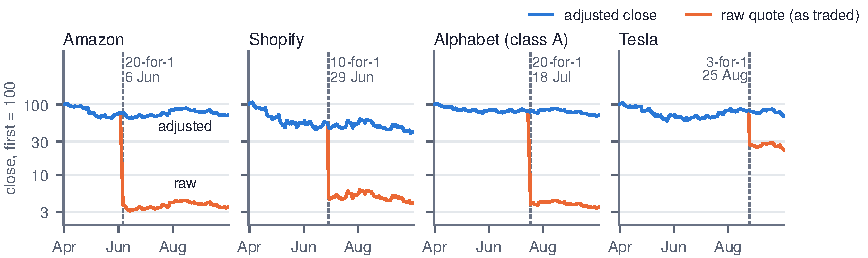
\includegraphics[width=\textwidth]{figures/real_panel}
\caption{The real-price panel: raw quotes (as traded) and adjusted closes of the four stocks,
each indexed to 100 at the first close, on a log scale. Every stock splits inside the window;
a program that ignores the split factors sees a one-day loss of 67\% to 95\%.}
\label{fig:real}
\end{figure*}

\section{Rule cards}
\label{app:cards}

\begin{table}[h]
\centering
\scriptsize
\input{cards_table}
\caption{Rule cards by family, the checks that verify each one, and whether the card names a
library call that follows the rule.}
\label{tab:cards}
\end{table}

\section{Task suite}
\label{app:tasks}

\begin{table}[h]
\centering
\footnotesize
\input{tasks_table}
\caption{The \NTaskAlgorithms{} algorithms of the task suite, with their split and the
one-step library call that solves them. Each algorithm has two tasks (variants a and b).}
\label{tab:tasks}
\end{table}
